\documentclass[11pt,a4paper]{article}

\usepackage{hyperref}
\usepackage{natbib}
\usepackage{times}
\usepackage{amsfonts}
\usepackage{amsmath}
\usepackage[psamsfonts]{amssymb}
\usepackage{amstext}
\usepackage{amsthm}
\usepackage{latexsym}
\usepackage{color}
\usepackage{graphicx}
\usepackage{subfigure}
\usepackage{subfiles}
\usepackage{enumerate}
\usepackage{algorithm}
\usepackage{algorithmic}
\usepackage{url}
\usepackage{dsfont}
\usepackage{xeCJK}
\usepackage{bm}
\usepackage{indentfirst}


%%%% The three packages below are about authors %%%%
\usepackage[T1]{fontenc}
\usepackage[utf8]{inputenc}
\usepackage{authblk}
%%%%%%%%%%%%%%%%%%%%%%%%%%%%%%%%%%%%%%%%%%%%%%%%%%%%

\usepackage[margin=1.2in]{geometry}

\makeatletter
\newtheorem*{rep@theorem}{\rep@title}
\newcommand{\newreptheorem}[2]{%
\newenvironment{rep#1}[1]{%
 \def\rep@title{#2 \ref{##1}}%
 \begin{rep@theorem}}%
 {\end{rep@theorem}}}
\makeatother

\hypersetup{
  colorlinks   = true,
  urlcolor     = blue,
  linkcolor    = blue,
  citecolor   = blue
}

% \def defines a new command. It does not check if
% the command already exists. If it exists, it will overwrite
\def\Cset{\mathbb{C}}
\def\Fset{\mathcal{F}}
\def\Hset{\mathcal{H}}
\def\Kset{\mathbb{K}}
\def\Pset{\mathbb{P}}
\def\Nset{\mathbb{N}}
\def\Qset{\mathbb{Q}}
\def\Rset{\mathbb{R}}
\def\Sset{\mathbb{S}}
\def\Xset{\mathcal{X}}
\def\Yset{\mathcal{Y}}
\def\Zset{\mathbb{Z}}
\def\Lagr{\mathcal{L}}
\def\Action{\mathcal{A}}

\let\Pr\undefined
\def\vcdim{\text{VCdim}}
\def\pdim{\text{Pdim}}


% DeclareMathOperator* defines a limit like command so 
% anything _{something} will appear under the command
\DeclareMathOperator*{\E}{\rm E}
\DeclareMathOperator*{\argmax}{\rm argmax}
\DeclareMathOperator*{\argmin}{\rm argmin}
\DeclareMathOperator{\sgn}{sgn}
\DeclareMathOperator{\supp}{supp}
\DeclareMathOperator{\last}{last}
\DeclareMathOperator{\Card}{Card}

\DeclareMathOperator*{\Prob}{\mathbb{P}}
\newcommand{\prob}{\text{Pr}}

\DeclareMathOperator{\sign}{sign}
\DeclareMathOperator{\range}{range}
\DeclareMathOperator{\rank}{rank}
\DeclareMathOperator{\diag}{diag}
\DeclareMathOperator{\Tr}{Tr}


\providecommand{\abs}[1]{\lvert#1\rvert}
\providecommand{\norm}[1]{\lVert#1\rVert}
\def\vcdim{\textnormal{VCdim}}


\newcommand{\G}{\mathcal{G}}
\newcommand{\cX}{{\mathcal X}}
\newcommand{\cY}{{\mathcal Y}}
\newcommand{\cA}{{\mathcal A}}
\newcommand{\cB}{{\mathcal B}}
\newcommand{\cF}{{\mathcal F}}
\newcommand{\cD}{\mathcal D}
\newcommand{\cH}{{\mathcal H}}
\newcommand{\mat}[1]{{\mathbf #1}}
\newcommand{\balpha}{\boldsymbol{\alpha}}
\newcommand{\bmu}{\boldsymbol{\mu}}

\newcommand{\w}{\mat{w}}
\newcommand{\x}{\mat{x}}
\newcommand{\X}{\mat{X}}

\newcommand{\sfp}{{\mathsf p}}
\newcommand{\sfq}{{\mathsf q}}
\newcommand{\Alpha}{{\boldsymbol \alpha}}
\newcommand{\Mu}{{\boldsymbol \mu}}
\newcommand{\bPsi}{\mat{\Psi}}
\newcommand{\bPhi}{{\mathbf \Phi}}
\newcommand{\scrH}{{\mathscr H}}
\newcommand{\hint}{\emph{hint}}

\renewcommand{\vec}[1]{\mathbf{#1}}

\providecommand{\norm}[1]{\| #1 \|}
\providecommand{\frobp}[2]{\langle#1, #2\rangle_F}
\def\dqed{\relax\tag*{\qed}}


\newtheorem{theorem}{Theorem}
\newreptheorem{theorem}{Theorem}
\newtheorem{lemma}[theorem]{Lemma}
\newreptheorem{lemma}{Lemma}
\newtheorem{definition}[theorem]{Definition}
\newtheorem{corollary}[theorem]{Corollary}
\newreptheorem{corollary}{Corollary}
\newtheorem{proposition}[theorem]{Proposition}
\newreptheorem{proposition}{Proposition}
\newtheorem{example}{Example}
\newreptheorem{example}{Example}



\title{Identification of Artist of Paintings}
\date{\vspace{-5ex}}
%\date{}  % Toggle commenting to test

\author[1]{Gyuhak Kim\thanks{gk1326@nyu.edu}}
\author[1]{YingYing Shi\thanks{gloriashiyy@nyu.edu}}
\author[2]{Yue Xiang\thanks{yue.xiang@nyu.edu}}
\affil[1]{Department of Mathematics, New York University}
\affil[2]{Department of Computer Science, New York University}

\renewcommand\Authands{ and }
\begin{document}




\maketitle
\begin{abstract}
This project adopted machine learning algorithms to classify the authors of paintings. We extracted features of paintings by convolutional neural network. The result shows that the algorithms are strong at identifying authors between different art movements such as Impressionism and Surrealism. The algorithms were still able to distinguish the most similar painters with fairly high precision.
\end{abstract}


\section{Introduction}
Recognizing the author of a painting is not easy for many people. Our project was inspired by the difficulty, and we hoped that machine learning could assist us on understanding arts. This report describes an approach to predicting the artist of a painting. This identification problem consists of two stages: feature extraction and classification. During our project, we perform an evaluation of possible feature extraction methods, as well performance of different classification algorithms. We believe that this technique could be extended to the field of aesthetics analysis and authentication. 

\section{Dataset}
Our dadtaset consists of 100 paintings for each painters. We have 11 painters, thus the total number of paintings is 1,1000. We separated the dataset into 65\% training, 15\% validation and 20\% testing. All paintings are downloaded from open source website WikiArt \cite{WikiArt}. We removed frames or distorted area in a painting. We further labeled our dataset into three subgroups by styles: Renaissance, impressionism and surrealism. The main reason for labeling the styles is to see the performance of the algorithms on differentiating similar paintings within the styles or between different styles.
Our 11 painters are the following: 
\vspace{0.1in}

\noindent 
{\small Impressionist: Claude Monet, Vincent van Gogh, Camille Pissarro, Pierre-Auguste Renoir, Alfred Sisley}

\noindent 
{\small Renaissance: Pietro Vannucci, Tintoretto, Titian, Sandro Botticelli }

\noindent 
{\small Surrealism: Rene Magritte, Salvador Dali}
\vspace{0.1in}

In Figure \ref{images}, we presented an example of paintings to emphasize the similarity and difference within and between the styles.
\begin{figure}
    \centering
    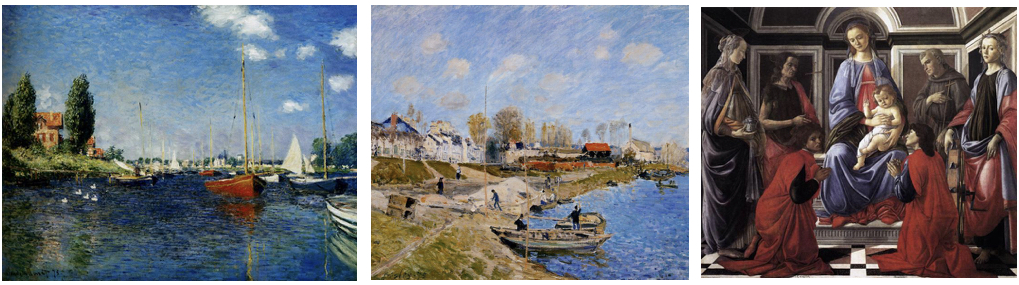
\includegraphics[width = 5in]{images}
    \caption{From left to right, \textit{Argenteuil}, \textit{Sand on the Quayside (Port Marly)}, and \textit{Madonna and Child with Six Saints} by Claude Monet, Alfred Sisley, Sandro Botticelli, respectively. Monet and Sisley are impressionists. They share similar themes and painting styles. On the other hands, Botticelli is from Renaissance. He usually illustrated stories from the Bible.}
    \label{images}
\end{figure}

\section{Feature Extraction}
We chose Caffe \cite{DBLP:journals/corr/DonahueJVHZTD13}, an open-source framework, and tried several convolutional neural network (CNN) architectures trained by different organizations. The architectures we tried include BVLC GoogleNet \cite{DBLP:journals/corr/DonahueJVHZTD13},  Fine-tuning on Flickr Style \cite{karayev2013recognizing}, BVLC AlexNet \cite{krizhevsky2012imagenet} since they aimed to classify by content, texture, or style. We chose the the architecture and layers with best performance, and it was evaluated by multiclass SVM.

We have chose BVLC GoogleNet as our final model. The BVLC GoogleNet of Caffe was trained on 1.2 million images into 1,000 leaf nodes. University of California, Berkeley, trained it to classify pictures by content. We investigated features from the second last level of the network, referred to as pool5/7x7s1. The reason to use the second last level is because it is of high dimension and well-trained after dozens of layers. Each picture is transferred to a 1024-dimensional vector and is computed from images center-cropped and re-sized to 256 by 256 pixels.

In order to illustrate features derived by deep learning, we performed principle component analysis (PCA) on our training set. The PCA result with three leading factors is presented in Figure \ref{pca_eig}. The first graph reveals that painters from different styles are highly separable. For example, we could expect that the artworks by Monet and Botticelli would be easily distinguishable as we saw in Figure \ref{images}. On the other hands, the second graph shows that painters from the same styles are hard to separate. This is because painters from the same art movements would share similar themes or styles. On the last graph, we can see the five impressionists painters are assorted, from which we could expect non-linear kernels or training models would be required for a better performance.

There were other feature extraction methods such as histogram of oriented gradients (HOG) or SIFT. Although deep learning is regarded as the state of the art method for image classification, we may find a combination of several feature extraction methods to improve the performance.

\begin{figure}
    \centering
        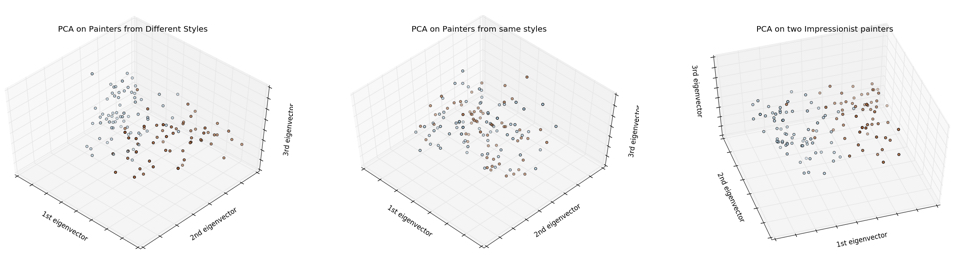
\includegraphics[width = 6in]{pca_eig.png}
        \caption{The first graph shows that it is separable between different styles. The second and third graph show that it is hardly separable within styles.}
        \label{pca_eig}
\end{figure}


\section{Learning Algorithms}
We implement several learning algorithms to distinguish between the whole classes: 11 artists, between different subclasses: 5 impressionist painters, 4 Renaissance painters and finally, between style: Impressionism, Renaissance and Surrealism. Based on our best performance of different method, we implement hard ensemble method. 

For linear classifier, we tried support vector machine (SVM) and linear discriminant analysis (LDA). Inspired by the paper \cite{DBLP:journals/corr/KarayevHWAD13}, we tried SVM with stochastic gradient descent to improve training speed. We chose hinge loss function and $l_2$ regularization. Since the features rarely had sparsity problem, $l_2$ regularization is used over $l_1$ regularization. We chose polynomial kernel of degree 2. The choice of degree can be explained by the PCA graph that shows quadratic boundary between different classes. Polynomials of degree higher than 2 were sensitive to overfitting.

For non-linear classifier, we used random forest (RF), k-nearest neighborhood (kNN), and quadratic discriminant analysis (QUA). For random forest, we restricted the choice of splitting variable to be the square root of 1024. Also, we chose the maximum depth of the tree to be 40. The depth of tree less than 40 were sensitive to overfitting. Also, 1000 number of trees were used in the forest.

Finally, hard voting ensemble method is used to improve prediction. Hard voting method decides the final prediction by the majority. For example, if two models vote for label A and one vote for label B, the final decision will be label A. We have chosen the three best classification models as the voting participants. They are SGD, SVM, and random forest. The other methods were discarded because their error rate was higher than 50 percent.

The ensemble method gives a slightly better result than the average of the participating models. We could obtain 2 percent lower error rate after ensemble method. Hard voting did not always give a better result than the single classification model. If a majority votes the wrong label, the prediction will be wrong. This explains why the ensemble method gave higher error rate than SVM when it classifies styles.

The reason why ensemble method does not give much higher prediction is that we only used three classification models in the voting process. In particular, if some of the models are similar, they are likely to miss the same pattern in the data, and the ensemble method will not be so different from the single classification model. We used SGD, SVM, and random forest in the voting. Since SGD and SVM are similar in techniques, they might overlook the same problem. The detailed error rate is presented in Table \ref{table1}.

\begin{table}[]
    \centering
    \begin{tabular}{ |c|c|c|c|c|c|c|c| } 
         \hline
          & SGD & SVM & kNN & LDA & QUA & RF & Ensenble \\ 
          \hline
         Whole dataset & 0.39 & 0.39 & 0.54 & 0.56 & 0.91 & 0.44 & 0.38 \\ 
         Impressionist & 0.24 & 0.32 & 0.42 & 0.37 & 0.76 & 0.27  & 0.24 \\ 
         Renaissance & 0.21 & 0.18 & 0.27 & 0.3 & 0.76 & 0.33 & 0.18 \\
         Style & 0.2 & 0.16 & 0.24 & 0.2 & 0.72 & 0.2 & 0.2 \\
         \hline
     \end{tabular}
    \caption{Error rate of each method. Impressionist (Renaissance) represents classification within the style. Style represents classification between styles.}
    \label{table1}
\end{table}



\section{Analysis}
We analyze our result by drawing a confusion matrix based on the prediction rate given by the ensemble method. A confusion matrix $M$ summarizes the performance of the final model and it is presented on right. For example, the entry $M_{21}$ detailed the frequency that a Monet painting is classified as Camille. Darker entry indicates a higher frequency.

The diagonal entries are relatively darker than the off-diagonal entries. This implies that each artist is mostly identified correctly by the final model. The confusion matrix is separated into 6 blocks by red lines. The diagonal block matrices show the model prediction within the same style while the off-diagonal block matrices show the prediction between different styles. Entries on the diagonal blocks are relatively darker than those on the off-diagonal blocks. This implies that the wrong predictions are usually occurred within the same style. 

The entry $M_{78}$ of the confusion matrix shows that the paintings by Tintoretto were misclassified frequently as those by Botticelli. The misclassification is explained by their similar painting styles and the themes they portray. Both artists drew religious stories or figures such as the Madonna or Evangelists from the Bible. The contents of the other Renaissance painters are slightly different. Titian usually drew portraits and Pietro painted the Madonna and child.

\begin{figure}
    \centering
    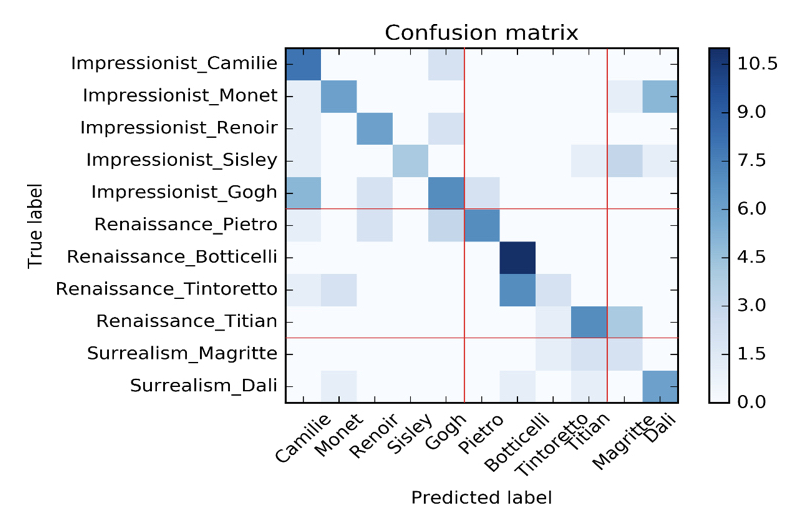
\includegraphics[width = 5in]{conf_mat}
    \caption{The diagonal entries are distinctly darker than the off-diagonals. This indicates that the prediction was fairly accurate.}
    \label{conf_mat}
\end{figure}

\section{Future Work}
There are three directions to improve the classification accuracy. The first is to increase the size of training set by collecting more paintings for each artist. The second is to try more classification models, then implement the ensemble method again. If we had more models in the ensemble method, the prediction accuracy would improve. The third is to try classification using part of the picture or picture with shade or distortions. We can apply this technique to practical recognition of paintings.


\bibliographystyle{abbrv}
\bibliography{my}

\end{document}
